\documentclass{article}

\usepackage[utf8]{inputenc}
\usepackage{t1enc}
\usepackage[magyar]{babel}
\sloppy

\usepackage{tikz}

\usepackage{amsthm}
\newtheorem{subproblem}{részfeladat}
\newtheorem*{reword}{Átfogalmazás}
\newtheorem*{answer}{Válasz}
\newtheorem*{subquestion}{Részkérdés}


\author{Endrey Márk}
\title{Ész Ventura\\98.~feladvány: Bonbonok\\\large Játssz bonbonnal, és nyerj csokit!}

\newcommand{\anz}[1]{$\mathrm{I}_{#1}$}
\newcommand{\nch}[1]{$\mathrm{II}_{#1}$}

\begin{document}
	\maketitle
	\tableofcontents
	\section{Elvek és építőelemek}
		\begin{subproblem}
			Egy bonbonos dobozban három sor bonbon található, minden sorban három bonbonnal. Bogi és Máté a négyzetrácsba rendezett kilenc bonbonból felváltva vehetnek el, egyszerre akár többet is az alábbi szabályok szerint. Az elvett bonbonoknak egy sorban vagy egy oszlopban kell lenniük, és egymással szomszédosak kell legyenek. Tehát el lehet venni akár egy egész sort, ha még teljes, vagy el lehet venni két egymás melletti bonbont, vagy egyet bárhonnan. Legalább egyet viszont kötelező elvenni, ha lehet. Aki utoljára vesz, az egy puszit kap. Bogi kezd. Tud úgy játszani, hogy mindenképpen puszit kapjon?
		\end{subproblem}

		\begin{reword}
			Adjunk általánosabb nevet Boginak és Máténak! Bogi a Kezdő Játékos, ,,die Anziehende'' (Spielerin), Máté pedig a ,,Követő'' (utánalépő) Játékos, ,,der Nachziehende'' (Spieler).
			Ezek a nevek (különösen a német megfogalmazás) sokat fognak segíteni majd a szimmetriaelvek felismerésében, megfogalmazásában.
			A játék természetétéből fakadóan nincs döntetlen stratégia, így vagy Kezdő, vagy Követő játékosnak van nyerési stratégiája.

			Kezdő Játékosnak van-e nyerő stratégiája, vagy Követő Játékosnak?
			A játék teljes fája nagyméretű --- $2\times2$-es táblaméret fölött már nem érdemes a teljes játékfát kimerítően felírni ---, de vannak-e elvek, tulajdonságok, algebrai vagy szimmetriaelvek, amelyek alapján a teljes fa felirása nélkül is megválaszolható a kérdés?
		\end{reword}

		\begin{answer}
			Az alábbi három szabály egyértelműen megadja a táblaméretből a választ:
			\begin{itemize}
				\item
				A $0\times n$ és $n\times0$ méretű tábla esetén nem a Kezdő Játékosnak játékosnak van nyerő stratégiája, hanem Követőnek:
				elfajuló eset, a játék eleve Kezdő Játékos vereségével már induláskor legott véget is ér.
				\item
				$m\times n$ méretű tábla esetén, ahol $m$ is és $n$ is pozitív (nemnulla) páros szám, szintén nincs a kezdő Játékosnak nyerő stratégiája,  hanem Követőnek van.
				\item
				$m\times n$ méretű tábla esetén, ahol $m$ is és $n$ közül legalább az egyik páratlan szám, a másik pedig pozitív (nemnulla) egyébként tetszőleges szám (akár páros, akár páratlan): ekkor pedig a Kezdő Játékosnak van nyerő stratégiája, nem Követőnek.
			\end{itemize}
			A továbbiakban a három szabálynak jelet adok: a ,,nulla-és-akármi'' szabály jele legyen ,,$\fbox{0n}$''-szabály, a ,,pozitív-páros-és-pozitív-páros'' szabály jele legyen ,,$\fbox{+0+0}$''-szabály, a ,,páratlan-és-akármi-pozitív'' szabály jele pedg legyen ,,\fbox{1+n}''-szabály.

			Előrebocsátom a szabályok bizonyításának sémáit is:
			\begin{itemize}
				\item $\fbox{0n}$
				\item $\fbox{+0+0} \to \mathbf{central}\,\,|\,\,\mathbf{decremental} \cdot \fbox{1+n}$
				\item $\fbox{1+n} \,\,\,\,\,\to \mathbf{axial}\,\,\,\,\,\,\,|\,\,\,\mathbf{decremental} \cdot \fbox{+0+0}$
			\end{itemize}
			Vagyis: a $\fbox{0n}$-szabály közvetlenül is igazolható.

			A $\fbox{1+n}$ kétféleképp is bizonyítható: vagy egyetlen lépésben egyfajta tengelyes szimmetriaelvre való hivatkozással, vagy pedig a tábla valamelyik oldalának eggyel való csökkentésével, afféle visszavezetéssel egy kisebb táblára, ami által a $\fbox{+0+0}$ esetre lépünk vissza.

			A $\fbox{+0+0}$-szabály is kétféleképp is bizonyítható: vagy egyetlen lépésben egyfajta középpontos szimmetriaelvre való hivatkozással, vagy pedig a tábla valamelyik oldalának eggyel való csökkentésével, afféle visszavezetéssel egy kisebb táblára, ami által a $\fbox{1+n}$ esetre lépünk vissza.

			A két utóbbi szabály tehát egymásra való kölcsönös visszavezetéssel igazolható, ahol a leszállás biztosan véges lépésben véget ét, de alternatívaként közvetlen egylépéses szimmetriaelvű bizonyításokat is használhatunk.
		\end{answer}

		\subsection{Kisméretű példák}

			A $0\times n$ eset egyértelműen üres táblát jelöl. Mivel innen Kezdő játékos eleve nem tud lépni, ezért tulajdonkép a játék anélkül, hoy egyetlen lépés is történnék, Kezdő Játékos vereségével véget ér. E szabály bizonyítása tehát igen egyszerű volt.

			A többi, nem-elfajuló esetet igazolásához már édemes kisebb táblarajzokat, játékforgatókönyveket felrajzolni.
			Az alább megrajzolt táblapéldákban Kezdő Játékos jele ,,I'', Követő Játékos jele pedig ,,II'' lesz, az indexelés pedig a lépések egymásutánját jelzi.

			Kezdjük a $2\times2$ táblából lehetséges játékok felrajzolásával, mert ez sok később is hasznosítható, általánosítható tanulságot nyújt.

			\subsubsection{A $2\times2$ eset mint később fontos általánosítási lehetőség}
				A ,,sortöltés'' mint kezdőlépés vereséghez vezet (márming ha Követő ezt kihsználja):\\
				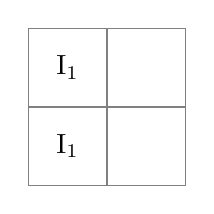
\begin{tikzpicture}
					\draw[step=1cm, color=gray] (-1, -1) grid (1, 1);
					\node at (-0.5, -0.5) {\anz1};
					\node at (-0.5,  0.5) {\anz1};
				\end{tikzpicture}
				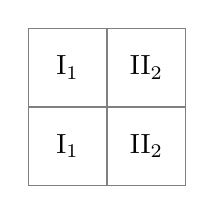
\begin{tikzpicture}
					\draw[step=1cm, color=gray] (-1, -1) grid (1, 1);
					\node at (-0.5, -0.5) {\anz1};
					\node at (-0.5,  0.5) {\anz1};
					\node at ( 0.5, -0.5) {\nch2};
					\node at ( 0.5,  0.5) {\nch2};
				\end{tikzpicture}
				A lényegesen különböző egyetlen alternatíva a ,,sarokkezdés'', ez viszont Követőt a ,,pepita'' válaszlépésre fogja kényszeríteni, mert ha Követő nem-pepitán reagálna, veszítene:\\
				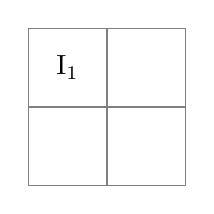
\begin{tikzpicture}
					\draw[step=1cm, color=gray] (-1, -1) grid (1, 1);
					\node at (-0.5,  0.5) {\anz1};
				\end{tikzpicture}
				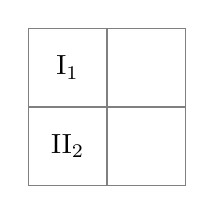
\begin{tikzpicture}
					\draw[step=1cm, color=gray] (-1, -1) grid (1, 1);
					\node at (-0.5,  0.5) {\anz1};
					\node at (-0.5, -0.5) {\nch2};
				\end{tikzpicture}
				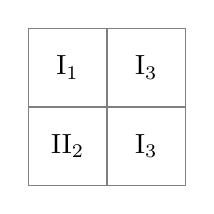
\begin{tikzpicture}
					\draw[step=1cm, color=gray] (-1, -1) grid (1, 1);
					\node at (-0.5,  0.5) {\anz1};
					\node at (-0.5, -0.5) {\nch2};
					\node at ( 0.5, -0.5) {\anz3};
					\node at ( 0.5,  0.5) {\anz3};
				\end{tikzpicture}

				Követőjátékos tehát  Kezdőjátékos ,,sarokkezdésére'' a ,,pepita'' válaszlépést fogja adni, innen pedig neki (Követőnek) nyerő sratégiája van:\\
				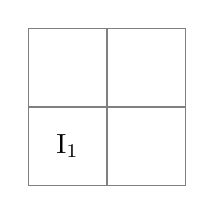
\begin{tikzpicture}
					\draw[step=1cm, color=gray] (-1, -1) grid (1, 1);
					\node at (-0.5, -0.5) {\anz1};
				\end{tikzpicture}
				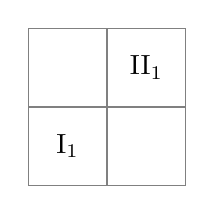
\begin{tikzpicture}
					\draw[step=1cm, color=gray] (-1, -1) grid (1, 1);
					\node at (-0.5, -0.5) {\anz1};
					\node at ( 0.5,  0.5) {\nch1};
				\end{tikzpicture}
				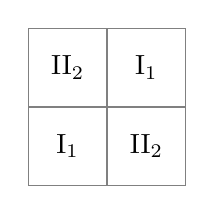
\begin{tikzpicture}
					\draw[step=1cm, color=gray] (-1, -1) grid (1, 1);
					\node at (-0.5, -0.5) {\anz1};
					\node at ( 0.5,  0.5) {\anz1};
					\node at ( 0.5, -0.5) {\nch2};
					\node at (-0.5,  0.5) {\nch2};
				\end{tikzpicture}

				Kezdőjátékosnak tehát sem a ,,sorkitöltős'', sem a ,,sarokkezdős'' kezsőlépéssel nincs nyerő stratégiája, más (lényegesen különböző, nem-ekvivalens) kezdőlépés pedig nem létezik ilyen kicsiny ($2\times2$-es) táblán. A $2\times2$-es játék tehát Követő számára nyújt nyerő stratégiát.

				Ezen a ponton érdemes észrevenni egy általánosítható gondolatot, egyfaja szimmetriaelvet. Követő Játékos számára az nyújt igen jól észben tartható nyerő stratégiát, ha mindenben majmolja a Kezdő Játékost! Precízebben fogalmazva: Követő Játékos tükrözze Kezdő Játékos friss lépését a tábla középpontjára (középpontos tükrözéssel), és lépjen szolgaian eszerint a stratégia szerint. A játékosok hivatalos német elnevezése véletlenül nagyon szépen lefesti épp ezt a stratégiát: ,,Anziehender'' és ,,Nachziehender''.

				Itt az alábbi dolgokat érdemes észrevenni:
				\begin{itemize}
					\item
					A $2\time2$-es tábla középpontja nem része a táblának (vagyis ez a középpont maga nem cella, hanem négy szomszédos cella közös sarkára esik. Tehát nem tartozik a tábla univerzumához. Ez nagyon fontos, ugyanis épp ez teszi lehetővé, hogy ,,der Nachziehende'', Követő Játékos mindig képes legyen ,,letükrözni'' a maga számára az ,,Anziehende'', vagyis Kezdő Játékos lépéseit. Ez nemcsak a $2\times2$-es, hanem a (nemnulla) párosszor párosas táblákra is igaz: a középpont nem része a tábla univerzumának. Viszont ha a tábla valamely oldala páratlan, akkor a középpont valós cella is egyben, ezért előfordulhat, hogy Követő Játékos nem képes letükrözni Kezdő Játékos lépését, mivel a középponton keresztül ez átfedést adna, ami lehetetlenné teszi a majomkodást. Épp ezért vonatkozik ez a bizonyítás szigorúan csak a (nemnulla) párosszor párosas táblákra.
				\end{itemize}
		\subsection{Abszolút elvek}
			\subsubsection{A középpontos tükrözés, nem-fizikai középpont}
			A párosszor párosas táblák esetében tehát a középpontos szimmetria révén általánosan is igazolni tudjuk Követő Játékos nyerési strtégiájának létezését.
			\subsubsection{A tengelyes tükrözés, fizikai tengely}
			A páratlanszor akármilyenes táblák esetében pedig Kezdő Játékosnak van nyerő stratégiája. A bizonyítás hasonló az előbbihez, de itt a tengelyes tükrözést használkuk ki, kicsit másképp. A trükk az, hogy Kezdő vágja ketté a legeslegelső lépésben a táblát két egyenlő részre azzal, hogy kiveszi a középső sort. Ezzel a tábla két teljesen szimmetrikus rész-táblára esik. Innen nézve Követő Játékos kerül rossz helyzetbe: Kezdőjátékos a saját második lépésétől  kezdve képes szimmetrikusan rákövetni Követő minden lépésére. A lényeg az, hogy tengelyes szimmetriát kell követnie. Kihasználja, ahogy a középső sor hiánya fizikai határt, ,,barrier''-t, kordont hoz létre a két táblafél között, így az átfedés nem tud bezavarni.
		\subsection{Visszalépés elv, relativitás}
		A visszalépéses elv akkor jön létre, ha KezdőJátékos legeslegelső lépéseként a táblázat valamely szélső sorát veszi ki. A bizonyítása a korábban mutatott jelöléses rövidítéses séma kölcsönös leszállása szerint végezhető.
	\section{Webalkalmazás}

		A nyerő stratégiák és a levezetési fák megtekinthetők az alábbi webalkalmazáson: \texttt{http://floor-plan-designer.curlgrep-phantom-funspec.hu:3000}

		A forráskód: \texttt{https://github.com/alignalghii/esz-ventura-98--bonbons}
\end{document}
